\documentclass{article}
\usepackage[utf8]{inputenc}

% \usepackage{listings}
\usepackage[utf8]{inputenc}
\usepackage{indentfirst}
\usepackage{graphicx}
\usepackage{hyperref}
\usepackage{caption}

\usepackage[linesnumbered,lined,commentsnumbered]{algorithm2e}
\usepackage{subcaption}
\usepackage{multirow}
\usepackage{amsmath}
\usepackage{xcolor}
\usepackage{wrapfig}
\usepackage{booktabs,caption,threeparttable}
\usepackage{amsfonts}
\usepackage{amssymb}
\usepackage{array}
\usepackage{xcolor}
\usepackage{wrapfig,lipsum,booktabs}
\usepackage[a4paper, total={6.5in, 8.5in}]{geometry}
\usepackage{setspace}
\usepackage{pdflscape}
\usepackage{tabu}
\usepackage{biblatex} %Imports biblatex package
\linespread{1.25}
\usepackage[breakable, theorems, skins]{tcolorbox}

% \tcbset{enhanced}

\graphicspath{ {./} }

\title{SEL}
\author{Vicol Valeriu}
\date{March 2022}


\begin{document}
% \bibliographystyle{plain}

\begin{titlepage}
    \centering
   \sc \LARGE
   \vspace{3cm}
   
\includegraphics[height=4cm,width=4cm]{media/logo.png}\\
   \vspace{1cm}
   Supervised and experiential learning\\ 

   \vfill
   \textbf{Practical Work 1}\\

   \vspace{2cm}
   \Large \vfill
   Valeriu Vicol 
   
   \vfill
 
  Barcelona, \today
\end{titlepage}
\thispagestyle{empty}
\tableofcontents
\vfill
\vspace{.75cm}
\setcounter{page}{1}
\newpage
\section{Introduction}
The purpose of this practical work is to gain practical knowledge  rule induction algorithms, in case of this work is the RISE
algorithm \cite{domingos1996unifying}, which represent a way of unifying the instance-based and rule-based induction
algorithms. Bellow we can find in depth descriptions of how current implementation is structure and why it is done in this way.
\section{Rise classifier}
Main concept of RISE is to create a set of rule from the instance and then try to extend the boundaries/constraints of the rules
in order to increase the precision of rules-set, the process is continuous until the precision is not increasing anymore.

\subsection{Structure}
In Figure \ref{fig:class_structure} we can see the class structure of the classifier, algorithm was implemented mainly 
using object-oriented programming \cite{rentsch1982object} style instead of keeping everything in array and there are few reasons for that. First
reason is that is easier to read for humans which is the most important thing for program, second is that if we would keep everything
in the array it would be hard to maintain the code and to extend it and also with object-oriented programming we can improve the 
performance of the code of the algorithm: 

\begin{itemize}
    \item \path{RiseClassifier}: represents the core class of algorithms which contains the classifier implementation with some 
    data processing functions
    \item \path{RiseUtils}: represents the utils class of algorithms which is computing distance between instance and rules, this logic
    was moved to another class instead of \path{RiseClassifier} as we can experiment with improvements and distances without touching the
    core logic of classifier.
    \item \path{Instance}: represent the instance from the dataset in OOP format
    \item \path{GenericInstanceAttribute}: represent an abstract class which define a property on the instance, we look at this 
    class like an contract definition which will be used across the program.
        \begin{itemize}
        \item \path{NumericalInstanceAttribute}: represent the concrete implementation, with some 
        logic related to numerical attributes of the instance.
        \item \path{CategoricalInstanceAttribute}: represent the concrete implementation, with some 
        logic related to categorical attributes of the instance, which are ordinal encoded beforehand.
        \end{itemize}
    \item \path{InstanceRule}: represent the rule inducted from instance class is similar to \path{Instance}
    except it has more utils method which are computing the distance and extending rule
    \item \path{GenericAttributeRule}: represent abstract class which define a concrete rule for concrete
    attribute
    \begin{itemize}
        \item \path{NumericalInstanceAttribute}: represent the concrete implementation, with some 
        logic related to numerical attributes of the instance.
        \item \path{CategoricalInstanceAttribute}: represent the concrete implementation, with some 
        logic related to categorical attributes of the instance, which are ordinal encoded beforehand.
        \end{itemize}
  \end{itemize}
 
\begin{figure}[htbp]
    \centering
    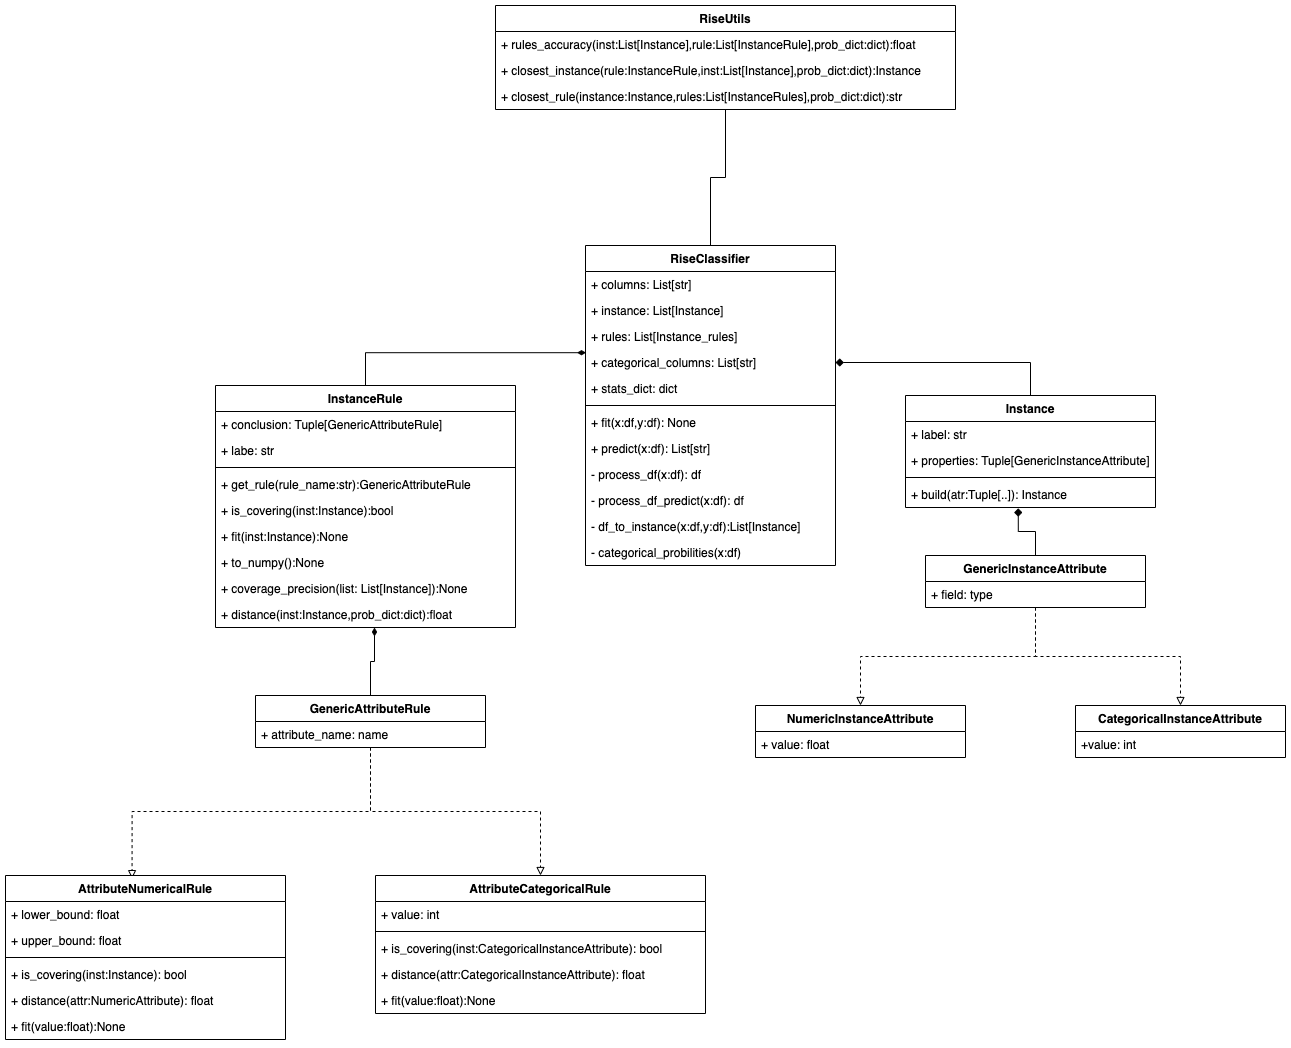
\includegraphics[width=0.9\textwidth]{media/sel.png}
    \caption{Rise classifier class structure}
    \label{fig:class_structure}
\end{figure}








\subsection{Implementation}
In current section we will discuss implementation of the algorithm
\begin{algorithm}[h!]
    \setlength{\algomargin}{0.5cm}
    \setstretch{1.15}
    \SetKwData{Left}{left}
    \SetKwData{This}{this}\SetKwData{Up}{up}
    \SetKwFunction{Union}{Union}
    \SetKwFunction{FindCompress}{FindCompress}
    \SetKwInOut{Input}{input}
    \SetKwInOut{Output}{output}
    \SetKwFor{While}{while}{:}{end}
    
    \Input{dataframe with the instances and dataframe with the labels}
    \Output{a set of rules inferred from the dataframe}
    \BlankLine
    
    normalization with min-max scaller, and ordinal encoding for categorical values\;
    $instances \gets$ \textbf{df\_to\_instances}$(dataframe,labels)$\;
    $stat\_dict \gets $ \textbf{categorical\_probabilites}$(dataframe,labels)$\;
    $rules \gets set([$InstanceRule$(it) $  for  $  it  $ in $ instances])$ \;
    $rules' \gets rules$\;
    $final\_precision \gets $ \textbf{rules\_precision}($rule,instances,stat\_dict)$\;
    \While{ True }{
        $intial\_precision \gets final\_precision$\;
        \ForEach{$index,rule \in$ \textbf{enum}($rules$)}{
            \If{$len(rules) < index$}{
                $break$ \# because during this loop we update $rules$ by removing some rules we have to add this 
                validation
            }
    
            $closest\_instance \gets$ \textbf{closest\_instance}($rule,instances,stat\_dict$)\;
            $rule ' \gets rule$\;
            $rule ' $.fit($closest\_instance$) \# most specific generalization\;
            $rules'[index] \gets rule'$\;
    
            \If{\textbf{rules\_precision}($instances,rules',..$)$\geq$\textbf{rules\_precision}($instances,rules,..$)}{
                \If{$rule' \in rules$}{
                    $rules' \gets rules' - rule'$\;
                }
                $rule \gets rules'$\;
            }
            \Else{
                $rules'[index] = rule$\;
            }
        }
        $final\_preicision \gets$\textbf{rules\_precision}($instances,rules,stats\_dict$)\;
        \If{$intial\_precision \geq final\_precion$}{
            $break$\;
        }
    
    }
    \caption{Rise classifier}
    \label{rise_alg}
\end{algorithm}

\newpage
\section{Datasets}
\subsection{Data processing}
\subsection{Wine}
\subsection{Breast cancer}
\subsection{earthquake}

\section{Conclusion}

% \addbibresource{refs.bib}



\end{document}